\documentclass[a4paper]{article}
\usepackage[T1]{fontenc}
\usepackage[utf8]{inputenc}
\usepackage[siunitx]{circuitikz}
\usepackage{siunitx}
\usepackage[margin=2cm]{geometry}
\usepackage{systeme}
\usepackage{mathtools}
\usepackage{wrapfig}
\usepackage[export]{adjustbox}
\usepackage{subcaption}
\usepackage{pdfpages}

\usepackage[swedish]{babel}
 % Needed for the Swedish characters

\title{Inlämningsuppgift 2-1045}
\author{Oskar Philipsson}
\index{}
\begin{document}

\begin{titlepage}
\maketitle

\end{titlepage}
\tableofcontents
\section{Intro}
\subsection{Uppgift}

\includepdf[pages={2}]{elektronikuppgifter.pdf}

\subsection{Avritat kretsschema}

\begin{figure}[h]
\begin{circuitikz}[american, scale=0.8, /tikz/circuitikz/bipoles/length=1cm] \draw
(0,0) to[sI=$i_0(t)$ ]++(0,4)
to[short,-*]node[label = A](A){}++(3,0)
--++(8,0) --++(0,-1)
node[transformer,anchor=A1](T){}
(T.A2) |- (3,0)node[label = B](B){}
to[short,*-]++(-3,0)
%(T.inner dot A1) node[circ]{}
%(T.inner dot B1) node[circ]{}

++(2,4) to[generic,l_=$Z_i$]++(0,-4)
++(2,4) to[R,l_=$R_1$,a^=1<\kilo\ohm>]++(0,-4)
++(3,4) to[R,l_=$R_2$,a^=1<\kilo\ohm>]++(0,-2)
to[C,l_=$C_1$,a^=2<\micro\farad>]++(0,-2)
++(3,4) to[C,l_=$C_2$,a^=1<\micro\farad>]++(0,-4)
;
\draw(T.B1)-- ++(0,1)--++(6,0)
to[L,l_=$L_1$,a^=10<\milli\henry>]++(0,-4)--++(-3,0)
to[R,l=$R_3$,a=10<\ohm>]++(0,4)
++(0,-4)--++(-3,0)--(T.B2)
(A) to[open] (B)
;
\end{circuitikz}
\caption{Avritat kretsschema}
\label{fig:orginal}
\end{figure}


\subsection{Symbolförklaringar}

\begin{figure}[h]
 
\begin{subfigure}{0.333\textwidth}
\begin{circuitikz} [american]\draw
(0,0) to[V,l^=$E_1$, a_=3<\volt>](4,0)
;
\end{circuitikz}
\caption{Spänningskälla}
\end{subfigure}
%
\begin{subfigure}{0.333\textwidth}
\begin{circuitikz} [american]\draw
(0,0) to[current source, l^=$I_{01}$,a_=1<\milli\ampere>](4,0)
;
\end{circuitikz}
\caption{Strömkälla}
\end{subfigure}
%
\begin{subfigure}{0.333\textwidth}
\begin{circuitikz} \draw
(0,0) to[R,l^=$R_2$,a_=2k](4,0)
;
\end{circuitikz}
\caption{Resistans}
\end{subfigure}
 
\end{figure}

Alla komponenter antas vara ideala. Spänningskällan har högre potential på sidan med plustecknet. Strömkällan driver en ström i pilens riktning. Komponenters värden betecknas med $E_n, I_{0n}, R_n$ för spänning, ström respektive resistans. Komponenternas värden står tydligt utmarkerade vid respektive komponent med dess värde på andra sidan komponenten.
Strömmen $I_n$ betecknar strömmen som går mellan två noder, förutom de som kommer direkt från en strömkälla vilka betecknas $I_{0m}$. Vardera strömm betecknas enbart en gång. 
Beteckningen $V_k$ används för potentialen i noden som beteckningen står vid.

\section{Förenkling av kretsschema}

Jag börjar med att ersätta strömkällan och dess inre resistans med en spänningskälla och den inre resistansen i serie. Detta får jag göra då de båda delkretsarna är antigen en Nortonekvivalent eller en Theveninekvivalent, vilket gör att kretsarna blir ekvivalenta. Sedan skriver jag om allt till komplex form och använder $j\omega$-metoden. Den omtalade spänningskällan får då värdet $E = Z_iI = 100e^{j\frac{\pi}{4}} \cdot 0.01 = e^{j\frac{\pi}{4}} V$ Detta illustreras i följande schema.


\begin{circuitikz}[american, scale=0.8, /tikz/circuitikz/bipoles/length=1cm] \draw
(0,0) to[esource ,v<=$E$]++(0,4)
to[generic,l_=$Z_i$,-*]++(3,0)node[label=A](A){}
--++(8,0) --++(0,-1)node(test){} 
node[transformer,anchor=A1](T){}
(T.A2) |- (3,0)node[label=B](B){}
to[short, *-](0,0)
%(T.inner dot A1) node[circ]{}
%(T.inner dot B1) node[circ]{}

++(5,4) to[generic,l_=$R_1$]++(0,-4)
++(2,4) to[generic,l_=$R_2$]++(0,-2)
to[generic,l_=$\frac{1}{j \omega C_1}$,a^=]++(0,-2)
++(3,4) to[generic,l_=$\frac{1}{j \omega C_2}$]++(0,-4)
;
\draw(T.B1)-- ++(0,1)--++(6,0)
to[generic,l_=$j \omega L_1$]++(0,-4)--++(-3,0)
to[generic,l=$R_3$]++(0,4)
++(0,-4)--++(-3,0)--(T.B2)

;
\end{circuitikz}


\begin{circuitikz}[american, scale=0.8, /tikz/circuitikz/bipoles/length=1cm] \draw
(0,0) to[esource ,v<=$E$]++(0,4)
to[generic,l_=$Z_i$,-*]++(3,0)node[label=A](A){}
--++(4,0) --++(0,-1)node(test){} 
node[transformer,anchor=A1](T){}
(T.A2) |- (3,0)node[label=B](B){}
to[short, *-](0,0)
%(T.inner dot A1) node[circ]{}
%(T.inner dot B1) node[circ]{}

++(5,4) to[generic,l_=$Z_{e1}$]++(0,-4)
;
\draw(T.B1)-- ++(0,1)--++(3,0)
to[generic,l_=$Z_t$]++(0,-4)
-|(T.B2)

;
\end{circuitikz}

\begin{circuitikz}[american, scale=0.8, /tikz/circuitikz/bipoles/length=1cm] \draw
(0,0) to[esource ,v<=$E$]++(0,4)
to[generic,l_=$Z_i$,-*]++(3,0)node[label=A](A){}
--++(4,0)
to[generic,l=$Z'_t$]++(0,-4) 
--(3,0)node[label=B](B){}
to[short, *-](0,0)
%(T.inner dot A1) node[circ]{}
%(T.inner dot B1) node[circ]{}

++(5,4) to[generic,l_=$Z_{e1}$]++(0,-4)
;

\end{circuitikz}




% Matris ekvation för nodpotentialerna.
\begin{equation*}
\begin{pmatrix}
\frac{1}{R_8} + \frac{1}{R_3} & 0 & 0 & -\frac{1}{R_3} & 0\\\\

0 & \frac{1}{R_5} + \frac{1}{R_2}  & -\frac{1}{R_5} & 0 & -\frac{1}{R_2}\\\\

0 & - \frac{1}{R_5} & \frac{1}{R_5} + \frac{1}{R_6} + \frac{1}{R_9} & 0 & -\frac{1}{R_6}\\\\

 -\frac{1}{R_3} & 0 & 0 & \frac{1}{R_4} + \frac{1}{R_3} + \frac{1}{R_7} & -\frac{1}{R_4}\\\\

0 & -\frac{1}{R_2} & -\frac{1}{R_6} & -\frac{1}{R_4} & \frac{1}{R_4} + \frac{1}{R_2} + \frac{1}{R_6}\\\\

\end{pmatrix}
 \begin{pmatrix}
    V_1\\\\
    V_2\\\\
    V_3\\\\
    V_4\\\\
    V_5\\\\
\end{pmatrix}
=
\begin{pmatrix}
    -I_{01} - I_{02}\\\\
    I_{02} - \frac{E_1}{R_2}\\\\
    0\\\\
    0\\\\
    \frac{E_1}{R_2}\\\\

\end{pmatrix}
\end{equation*}

Om vi sätter in värdena och mulitplicerar båda sidor med 1000 fås följande (skalärerna har avrundats till 5 decimaler för att inte ta för stor plats i detta dokument. Alla värden behölls från början till slut i matlab för att ha maximal precision.)

%Numerisk ekvation där båda sidor multiplicerats med 1000 och avrundats till 5 decimaler.
\begin{equation*}
\begin{pmatrix}
0.45833&0&0&-0.33333&0\\
0&0.7&-0.2&0&-0.5\\
0&-0.2&0.47778&0&-0.16667\\
-0.33333&0&0&0.72619&-0.25\\
0&-0.5&-0.16667&-0.25&0.91667\\

\end{pmatrix}
 \begin{pmatrix}
    V_1\\
    V_2\\
    V_3\\
    V_4\\
    V_5\\
\end{pmatrix}
=
\begin{pmatrix}
-3\\
0.5\\
0\\
0\\
1.5\\

\end{pmatrix}
\end{equation*}

Efter lösning av systemet i matlab erhålls följande potentialer. 
\begin{equation*}
    \systeme{
V_1 = -8.27672,
V_2 = 4.62117,
V_3 = 3.37195,
V_4 = -2.38050,
V_5 = 4.12086
    }
\end{equation*}
Vi får då tomgångsspänningen till $E_2 + V_3 = 9.37195\si{\milli\volt}$. 


\section{Bestämning av kortslutningsströmmen}

Nu till att bestämma kortslutningströmmen. Uppdaterat diagram efter kortslutning.

\begin{circuitikz}[american, scale=0.8, /tikz/circuitikz/bipoles/length=1cm] \draw
(4,0) -- (0,0)node[label={below:$V_1$}] {} to[current source,*-* ,l^=$I_{02}$,a_=2<\milli\ampere>, i=$I_{02}$]++(0,4)node[label={left:$V_2$}]{}
to[V,l^=$E_1$, a_=3<\volt>,i=$I_8$, invert]++(4,0)
to[R,l^=$R_2$,a_=2k,-*]++(4,0)node[label={above:$V_5$}]{}
to[R,l^=$R_6$,a_=6k, i=$I_7$]++(4,0)
to[R,l^=$R_9$,a_=9k,i_<=$I_4$]++(0,-4)
to[R,l^=$R_7$,a_=7k, -*,i>_=$I_3$]++(-4,0)node[label={below:$V_4$}]{}
to[R,l^=$R_3$,a_=3k, i=$I_5$]++(-4,0) -- ++(0,-4)
to[current source, l^=$I_{01}$,a_=1<\milli\ampere>,i=$I_{01}$]++(8,0) node[ground]{} 
-- ++(0,4)
++(0,-2) to[R,l^=$R_8$,a_=8k,i>_=$I_2$]++(-8,0)
++(-4,6) -- ++(0,2)
to[R,l^=$R_5$,-*,a_=5k, i=$I_9$]++(12,0)node[label={above:$V_3$}]{}-- ++(0,-2)--++(1,0)
to[R,l^=$R_{10}$,a_=10k,i>^=$I_{10}$]++(2,0)
to[V, invert, l^=$E_2$,a=6<\volt>, -o]++(2,0)node[anchor=west]{A}
to[short]++(0,-4)node[anchor=west]{B} 
to[short, o-]++(-5,0)
++(-4,0)to[R,l^=$R_4$,a_=4k,i>_=$I_6$]++(0,4)
;
\end{circuitikz}

Skillnaden är att vi nu har en ny positiv ström $I_{10}$ som går ifrån noden $V_3$ och är vår kortslutningsström vi söker. För att finna denna gör vi om nodanalysen på den kortslutna kretsen.

\begin{align*}
NOD 1: \ &  I_{01}  - I_2 - I_5 + I_{02} = 0\\
NOD 2: \ &  I_9  - I_8 - I_{02} = 0\\
NOD 3: \ &  -I_9 - I_7 - I_4 + I_{10}= 0\\
NOD 4: \ &  I_6  + I_5 - I_3  = 0\\
NOD 5: \ &  I_7  + I_8 - I_6 = 0\\
\end{align*}


\begin{equation*}
    \systeme{
 I_{01} + I_{02} - \frac{0-V_1}{R_8} - \frac{V_4 - V_1}{R_3}= 0,
\frac{V_2 - V_3}{R_5} - \frac{V_5 - V_2 - E_1}{R_2} - I_{02} = 0,
\- \frac{V_2 - V_3}{R_5} - \frac{V_5 - V_3}{R_6} - \frac{0 - V_3}{R_9} + \frac{V_3 -(-E_2)}{R_{10}}= 0,
\frac{V_4 - V_5}{R_4} + \frac{V_4 - V_1}{R_3} - \frac{0-V_4}{R_7}= 0,
\frac{V_5 - V_3}{R_6} + \frac{V_5 - V_2 - E_1}{R_2} - \frac{V_4 - V_5}{R_4}= 0
}
\end{equation*}


% Matris ekvation för nodpotentialerna.
\begin{equation*}
\begin{pmatrix}
\frac{1}{R_8} + \frac{1}{R_3} & 0 & 0 & -\frac{1}{R_3} & 0\\\\

0 & \frac{1}{R_5} + \frac{1}{R_2}  & -\frac{1}{R_5} & 0 & -\frac{1}{R_2}\\\\

0 & - \frac{1}{R_5} & \frac{1}{R_5} + \frac{1}{R_6} + \frac{1}{R_9} + \frac{1}{R_{10}} & 0 & -\frac{1}{R_6}\\\\

 -\frac{1}{R_3} & 0 & 0 & \frac{1}{R_4} + \frac{1}{R_3} + \frac{1}{R_7} & -\frac{1}{R_4}\\\\

0 & -\frac{1}{R_2} & -\frac{1}{R_6} & -\frac{1}{R_4} & \frac{1}{R_4} + \frac{1}{R_2} + \frac{1}{R_6}\\\\

\end{pmatrix}
 \begin{pmatrix}
    V_1\\\\
    V_2\\\\
    V_3\\\\
    V_4\\\\
    V_5\\\\
\end{pmatrix}
=
\begin{pmatrix}
    -I_{01} - I_{02}\\\\
    I_{02} - \frac{E_1}{R_2}\\\\
    -\frac{E2}{R_{10}}\\\\
    0\\\\
    \frac{E_1}{R_2}\\\\

\end{pmatrix}
\end{equation*}
 
Samma ide som förra gången. Efter att ha satt in siffror fås.


\begin{equation*}
\begin{pmatrix}
0.45833&0&0&-0.33333&0\\
0&0.7&-0.2&0&-0.5\\
0&-0.2&0.57778&0&-0.16667\\
-0.33333&0&0&0.72619&-0.25\\
0&-0.5&-0.16667&-0.25&0.91667\\
\end{pmatrix}
 \begin{pmatrix}
    V_1\\
    V_2\\
    V_3\\
    V_4\\
    V_5\\
\end{pmatrix}
=
\begin{pmatrix}
-3\\
0.5\\
-0.6\\
0\\
1.5\\
\end{pmatrix}
\end{equation*}

Potentialerna blir denna gång.

\begin{equation*}
    \systeme{
    V_1 = -9.12689,
    V_1 = 2.10687,
    V_1 = 2.27034,
    V_1 = -3.54948,
    V_1 = 1.85881
    }
\end{equation*}


Från detta får vi $$I_{10} = \frac{V_3 + E_2}{R_{10}} = 0.62270\si{\milli\ampere}$$


\section{Theveninekvivalent}

En generell Theveninekvivalent

\begin{circuitikz}[american, scale=0.8, /tikz/circuitikz/bipoles/length=1cm] \draw
(0,0)node[anchor=west]{B} to[short, o-] ++(-4,0)
to[voltage source, invert, l= $E$]++(0,4)
to[R,l=$R$,-o]++(4,0)node[anchor=west]{A}
;
\end{circuitikz}

Där $E$ är tomgångsspänningen och $R$ är inre resistansen i orginalkretsen. $R$ beräknas genom $R = U/I = 15.05043 \si{\kilo\Omega}$ ($I$ är kortslutningsströmmen).

\section{Svar}

\begin{circuitikz}[american, scale=0.8, /tikz/circuitikz/bipoles/length=1cm] \draw
(0,0)node[anchor=west]{B} to[short, o-] ++(-4,0)
to[voltage source,invert, l= $E$, a=9.372<\volt>]++(0,4)
to[R,l=$R$,a=15.05<\kilo\Omega>,-o]++(4,0)node[anchor=west]{A}
;
\end{circuitikz}

\end{document}